\chapter{Analyse-Klassen-Diagramm}

In diesem Kapitel wird zuerst auf die Klassen, welche für die Implementierung nötig sind, eingegangen bevor die Abhängigkeiten zwischen diesen Klassen nochmal übersichtlich mittel eines Analyse-Klassen-Diagramms dargestellt werden.

\section{Klassen}
\begin{multicols}{2}
\begin{itemize}
    \item Kunde
    \item Adresse
    \item Vertrag
    \item Mitarbeiter
    \item Rolle
    \item Buchung
    \item Fahrzeug
    \item Fahrzeugklasse
    \item Bild
    \item Reifensatz
    \item Reifen
    \item Kennzeichen
    \item Ausrüstung
    \item Rechnung
    \item Mahnung
    \item Standort
    \item Filiale
    \item Rabattaktion
    \item Backup
\end{itemize}
\end{multicols}

\newpage

\section{Diagramm}

\begin{figure}[!ht]
    \centering
    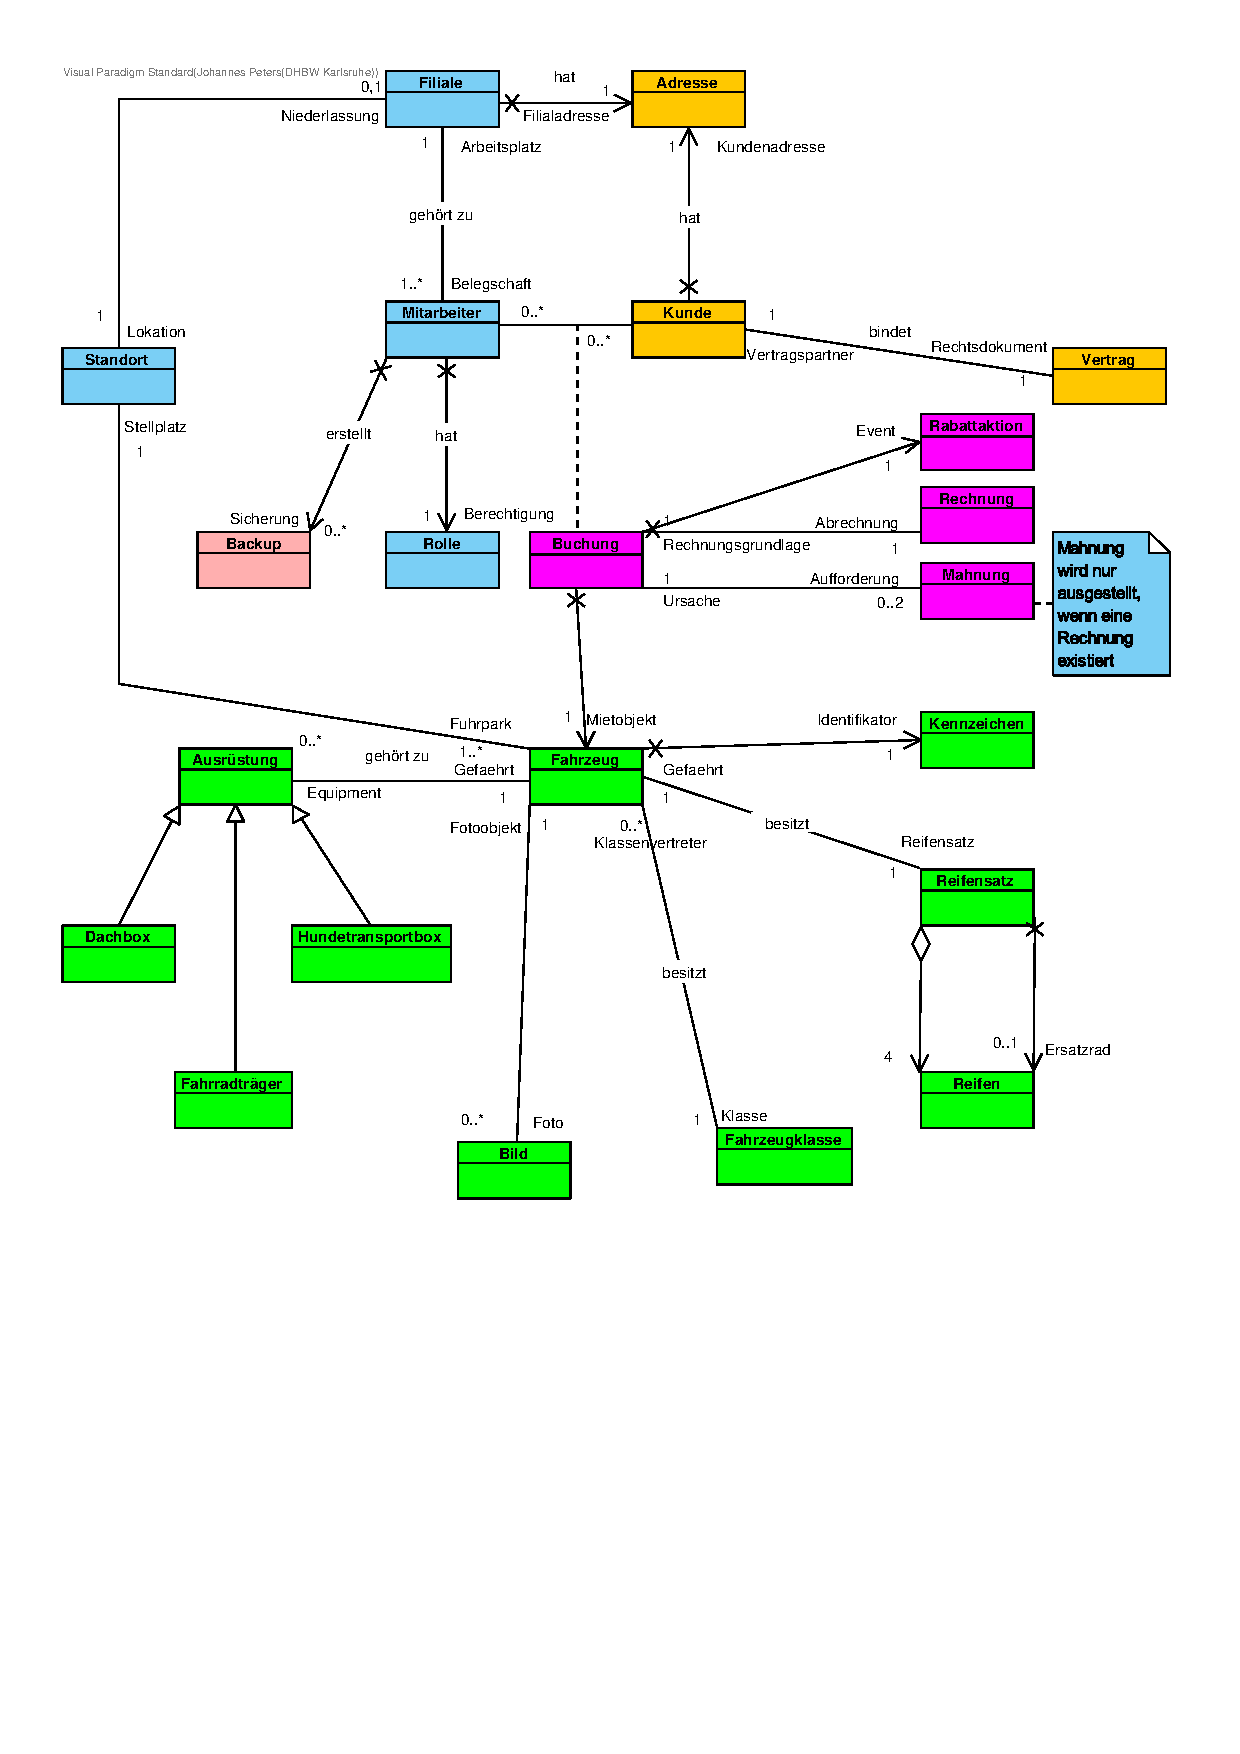
\includegraphics[width=\textwidth, trim = 0cm 10cm 0cm 0cm]{Bilder/Diagramme/Analyseklassendiagramm.pdf}
    \caption{Analyseklassendiagramm}
    \label{img:akd}
\end{figure}